%% IFBThesis Latex Template Version 1.0, a fork of :
%% 	RiSE Latex Template - version 0.5
%%
%% IFBthesis latex template for thesis and dissertations
%% https://github.com/auyer/IFBtcc
%%
%% (c) 2017 Rafael de Campos Passos (rcpassos@ieee.org)
%%
%% This document was initially based on RiSE Latex template, from Yguaratã
%% Cerqueira Cavalcanti
%%
%% GENERAL INSTRUCTIONS
%%
%% We strongly recommend you to compile your documents using pdflatex command.
%% It is also recommend use the texlipse plugin for Eclipse to edit your documents.
%%
%% Options for \documentclass command:
%%         * Idiom
%%           pt   - Portguese (default)
%%           en   - English
%%
%%         * Text type
%%           bsc  - B.Sc. Thesis
%%           msc  - M.Sc. Thesis (default)
%%           qual - PHD qualification (not tested yet)
%%           prop - PHD proposal (not tested yet)
%%           phd  - PHD thesis
%%
%%         * Media
%%           scr  - to eletronic version (PDF) / see the users guide
%%
%%         * Pagination
%%           oneside - unique face press
%%           twoside - two faces press
%%
%%		   * Line spacing
%%           singlespacing  - the same as using \linespread{1}
%%           onehalfspacing - the same as using \linespread{1.3}
%%           doublespacing  - the same as using \linespread{1.6}
%%
%% Reference commands. Use the following commands to make references in your
%% text:
%%          \figref  -- for Figure reference
%%          \tabref  -- for Table reference
%%          \eqnref  -- for equation reference
%%          \chapref -- for chapter reference
%%          \secref  -- for section reference
%%          \appref  -- for appendix reference
%%          \axiref  -- for axiom reference
%%          \conjref -- for conjecture reference
%%          \defref  -- for definition reference
%%          \lemref  -- for lemma reference
%%          \theoref -- for theorem reference
%%          \corref  -- for corollary reference
%%          \propref -- for proprosition reference
%%          \pgref   -- for page reference
%%
%%          Example: See \chapref{chap:introduction}. It will produce
%%                   'See Chapter 1', in case of English language.
%%
%% Citation commands:
%%          \citet (from natbib) -- To cite a reference as part of the narrative
%%          \citep (from natbib) -- To cite a reference between parenthesis
%%          citationblock environment -- To produce direct citation blocks according to the ABNT

\documentclass[pt,twoside,onehalfspacing,bsc]{ifgtcc}

\usepackage{colortbl}
\usepackage{color}
\usepackage[table]{xcolor}
\usepackage{microtype}
\usepackage{bibentry}
\usepackage{subfigure}
\usepackage{multirow}
\usepackage{rotating}
\usepackage{booktabs}
\usepackage{pdfpages}
\usepackage{caption}
\usepackage{lipsum}
\usepackage{sectsty}
%pages
\usepackage{lastpage}
\usepackage{float}
\usepackage{amsmath,amssymb,amsfonts}
\usepackage{algorithmic}
\usepackage{graphicx}
\usepackage{textcomp}
\usepackage{xcolor}
\usepackage{authblk}
\usepackage{tikz-cd}
\usepackage{listings}
\usepackage{mathtools}
\usepackage{float}
\usepackage{caption}
%% Set the language used in your code in the block above

\captionsetup[table]{position=top,justification=centering,width=.85\textwidth,labelfont=bf,font=footnotesize}
\captionsetup[lstlisting]{position=top,justification=centering,width=.85\textwidth,labelfont=bf,font=footnotesize}
\captionsetup[figure]{position=bottom,justification=centering,width=.85\textwidth,labelfont=bf,font=footnotesize}

%% Chapter and (Sub)Section fonts must be same size as text (12)
\sectionfont{\fontsize{12}{15}\selectfont}
\subsectionfont{\fontsize{12}{15}\selectfont}
\subsubsectionfont{\fontsize{12}{15}\selectfont}

%% Change the following pdf author attribute name to your name.
\usepackage[linkcolor=black,
            citecolor=black,
            urlcolor=black,
            colorlinks,
            pdfpagelabels,
            pdftitle={Rise Thesis Template (ABNT)},
            pdfauthor={Rise Thesis Template (ABNT)},
            breaklinks=true]{hyperref}

\address{FORMOSA}

\universitypt{Instituto Federal de Goiás}
\universityen{Federal Institute of Goi\'as}

\campus{{\it Campus} Formosa}

\departmentpt{Departamento de Áreas Acadêmicas}
\departmenten{Academic Department}

\programpt{Análise e Desenvolvimento de Sistemas}
\programen{Systems Analyses and Develpment}

\majorfieldpt{Ciência da Computação}
\majorfielden{Computer Science}

\title{Meu TCC}

\date{2019}

\author{Aluno da Silva}
\adviser{Prof. Dr. Waldeyr Mendes Cordeiro da Silva}
%\coadviser{Nome dompleto do co-orientador }

% Macros (defines your own macros here, if needed)
\def\x{\checkmark}
%\let\lstlistoflistings\origlstoflistings
\begin{document}

\frontmatter

\frontpage

\presentationpage

\begin{fichacatalografica}
\FakeFichaCatalografica % Comment this line when you have the correct file
%\includepdf{fig_ficha_catalografica.pdf} % Uncomment this
\end{fichacatalografica}


%NAO APAGAR ISSO AQUI
%\banca

\begin{ata}
\begin{figure}
	\centering 
	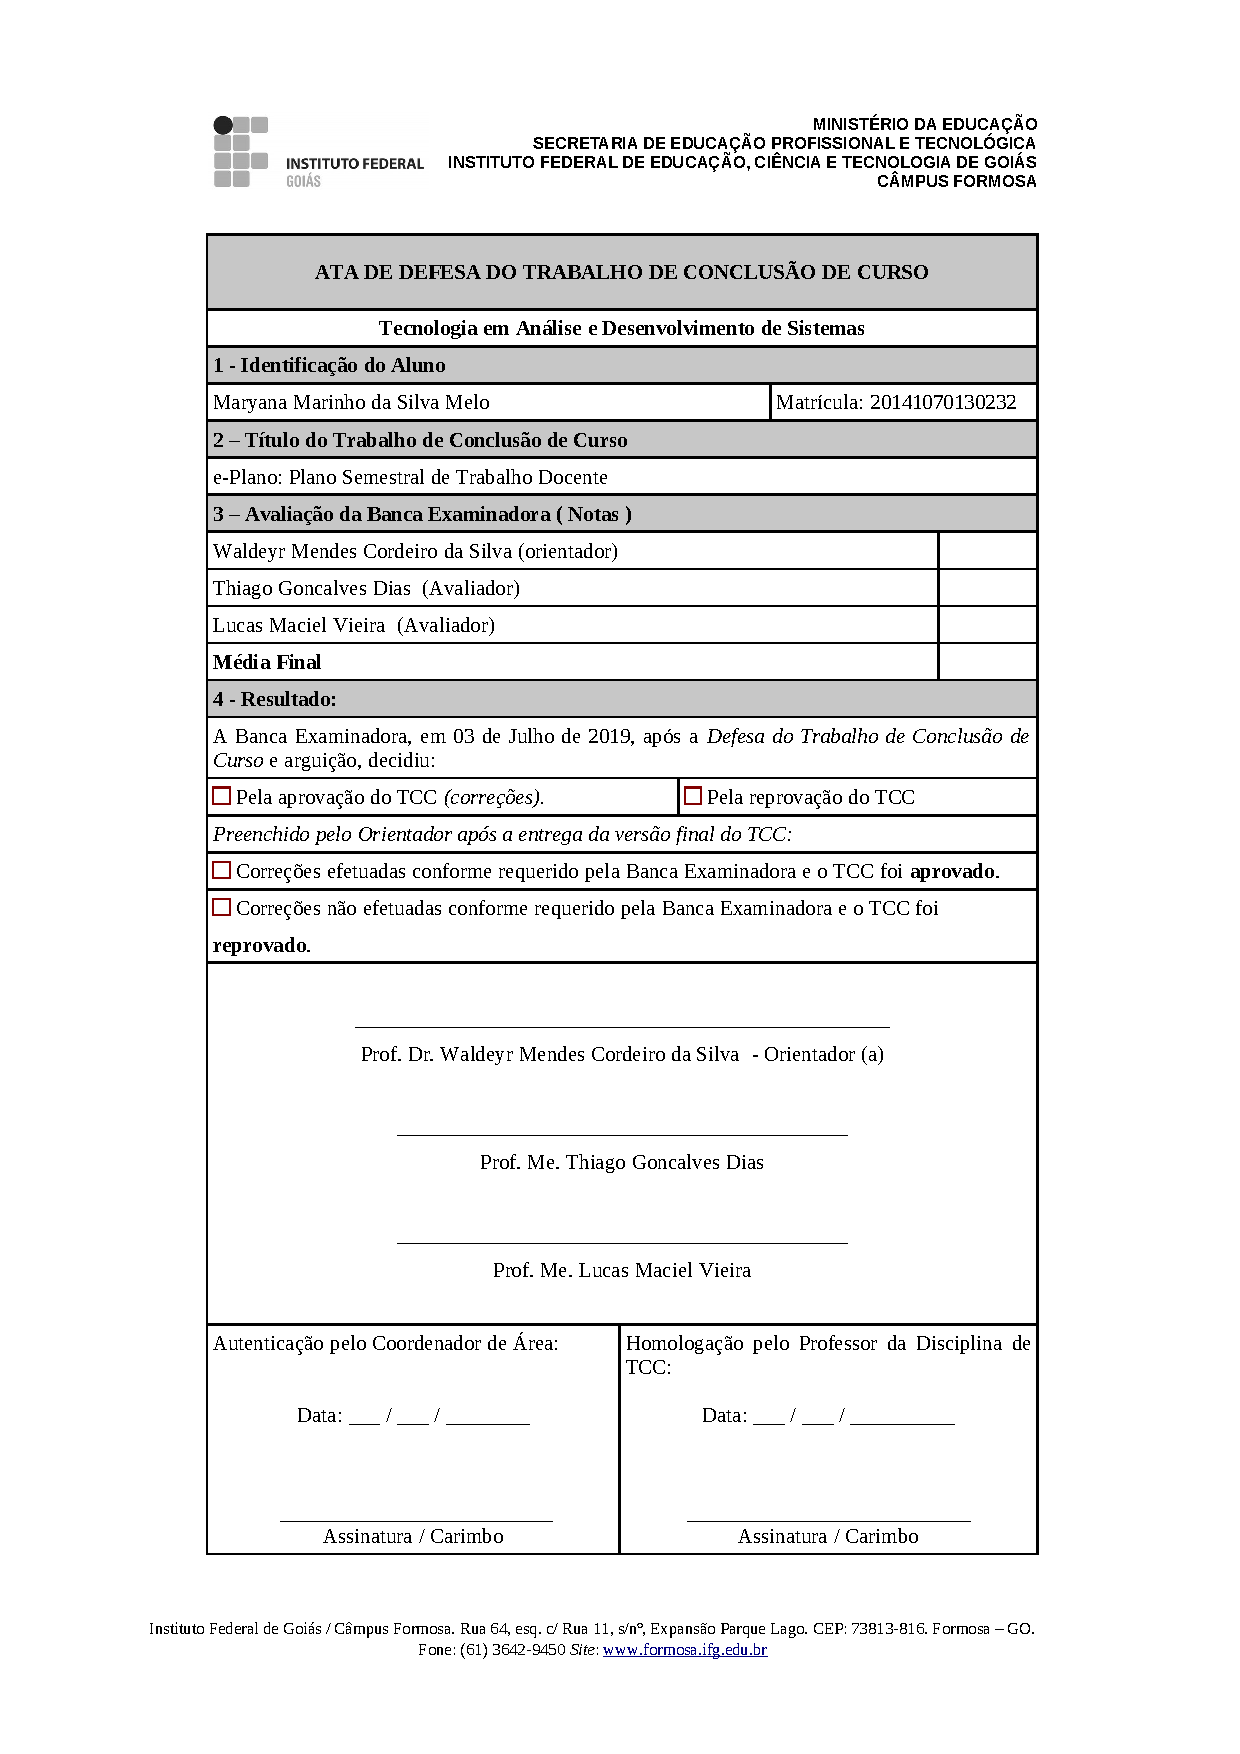
\includepdf[pages=-,width=\textwidth]{doc/ModeloAta.pdf}
\end{figure}
\end{ata}


\begin{ata}
	\begin{figure}
		\centering 
		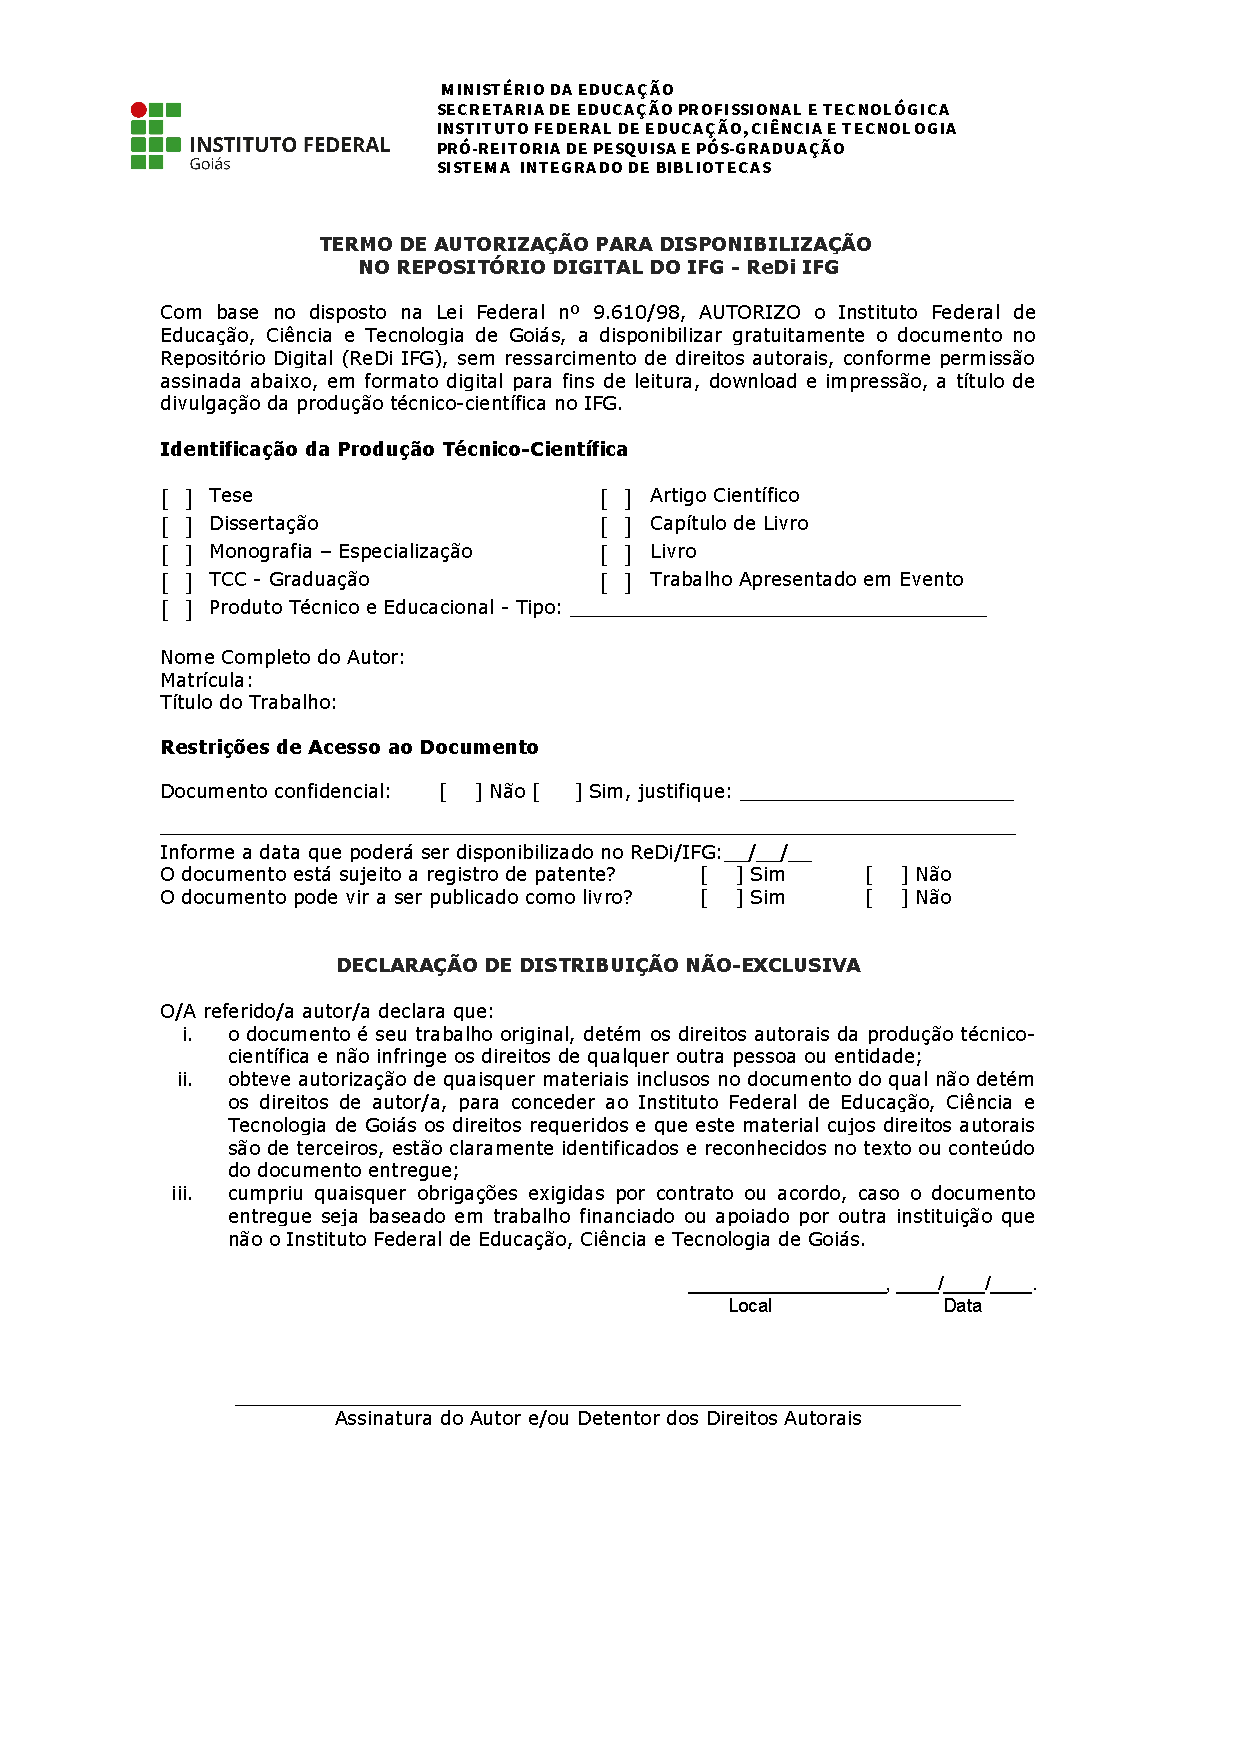
\includepdf[pages=-,width=\textwidth]{doc/redi.pdf}
	\end{figure}
\end{ata}


\begin{dedicatory}
Eu dedico ...
\end{dedicatory}

% \acknowledgements
% \lipsum[1-4]

Agradeço a minha mãe por me apoiar sempre, e por fazer eu chegar ate aqui. Sem ela não seria possível.
Ao meu orientador professor Dr. Waldeyr Mendes Cordeiro da Silva, pelo conhecimento, orientação e compreensão.
Aos meus amigos pelo apoio, incentivo e torcida pelo meu sucesso.
A todos que me ajudaram direta ou indiretamente nessa nessa jornada. 


% \begin{epigraph}[]{Márcio de Deus}
% When one finds a hard problem, the more complicated it is, the more one ought to work towards enlightening it's solution.
% \end{epigraph}

\resumo
% Escreva seu resumo no arquivo resumo.tex
{\parindent0pt
	Caminhos metabólicos definem coletivamente o repertório bioquímico de um organismo assim como os métodos pelos quais esse organismo produz seus produtos químicos. Os caminhos metabólicos têm sido reconstruídos usando uma larga variedade de métodos computacionais e fonte de dados, incluindo dados  {\it -omics} e restrições tais como a presença de enzimas, estequeometria e termodinâmica. A reconstrução de cada caminho em relação ao outro pode variar por alguns aspectos, como a granularidade dos detalhes bioquímicos. A demonstração de reações químicas utilizando a reescrita de grafos é um método que possibilita apresentar os produtos iniciais, finais e intermediários por meio da modelagem dos caminhos como hiperfluxos inteiros. Neste trabalho, foram esboçadas as reescritas de grafos as quais descrevem reações cíclicas catalisadas pela sintase dos terpenos das plantas para produzir monoterpenos, sendo também gerado o espaço químico possível para explorar o potencial da sintase de monoterpenos. Nesse sentido, é fornecida uma interface gráfica com objetivo de facilitar a criação dos códigos de simulação.

\begin{keywords}
	caminhos metabólicos, monoterpenos, biossíntese, plantas, reescrita de grafos
\end{keywords}
}

\abstract
% Write your abstract in a file called abstract.tex
{\parindent0pt
	O abstract é o resumo em língua Inglesa. 
Embora o conteúdo apresentado seja o mesmo, não deve ser a tradução literal.

\begin{keywords}
TCC, IFG, model
\end{keywords}
}

% List of figures
\listoffigures

% List of Codes
%\lstlistoflistings

% List of tables
\listoftables

% List of acronyms
% Acronyms manual: http://linorg.usp.br/CTAN/macros/latex/contrib/acronym/acronym.pdf
\listofacronyms
\begin{acronym}[ACRONYM] 
% Não é necessário ordenar as siglas
\acro{IFG}[IFG]{Instituto Federal de Educação, Ciência e Tecnologia de Goiás}
\acro{DAA}[DAA]{Departamento de Áreas Acadêmicas}
\acro{Cefet}[Cefet]{Centros Federais de Educação Profissional e Tecnológica}
\acro{Uneds}[Uneds]{Unidade de Ensino Descentralizada}
\acro{ETFG}[ETFG]{Escola Técnica Federal de Goiás}
\acro{URL}[URL]{Uniform Resource Locator}
\acro{HTML}[HTML]{Hypertext Markup Language}
\acro{CSS}[CSS]{Cascading Style Sheets}
\acro{SGBDs}[SGBDs]{Sistema de Gerenciamento de Banco de Dados}
\acro{SQL}[SQL]{Structured Query Language}
\acro{NoSQL}[NoSQL]{Not Only SQL}
\acro{REST}[REST]{Representational State Transfer}
\acro{HTTP}[HTTP]{Hypertext Transfer Protocol}
\acro{URI}[URI]{Uniform Resource Identifier}
\acro{JSON}[JSON]{JavaScript Object Notation}
\acro{PDF}[PDF]{Portable Document Format}
%%
\acro{afm}[AFM]{Alphabet Frequency Matrix}
\acro{api}[API]{Application Programming Interface}
\acro{arima}[ARIMA]{Auto-Regressive Integrated Moving Average}
\acro{brn}[BRN]{Bug Report Network}
\acro{bts}[BTS]{Bug Triage System}
\acro{cas}[CAS]{Context-Aware Systems}
\acro{ccb}[CCB]{Change Control Board}
\acro{cr}[CR]{Change Request}
\acro{cvs}[CVS]{Concurrent Version System}
\acro{es}[ES]{Expert System}
\acro{floss}[FLOSS]{Free/Libre Open Source Software}
\acro{glr}[GLR]{Generalized Linear Regression}
\acro{gqm}[GQM]{Goal Question Metric}
\acro{html}[HTML]{HyperText Markup Language}
\acro{ir}[IR]{Information Retrieval}
\acro{irt}[IRT]{Recôncavo Institute of Technology}
\acro{jdt}[JDT]{Jazz Duplicate Finder}
\acro{lda}[LDA]{Latent Dirichlet Allocation}
\acro{loc}[LOC]{Lines of Code}
\acro{lsi}[LSI]{Latent Semantic Indexing}
\acro{ms}[MS]{Mapping Study}
\acro{msr}[MSR]{Mining Software Repositories}
\acro{nlp}[NLP]{Natural Language Processing}
\acro{promise}[PROMISE]{Predictive Models in Software Engineering}
\acro{rbes}[RBES]{Rule-Based Expert System}
\acro{rhel}[RHEL]{RedHat Enterprise Linux}
\acro{saas}[SaaS]{Software as a Service}
\acro{scm}[SCM]{Software Configuration Management}
\acro{serpro}[SERPRO]{Brazilian Federal Organization for Data Processing}
\acro{slr}[SLR]{Stepwise Linear Regression}
\acro{slr}[SLR]{Systematic Literature Review}
\acro{svd}[SVD]{Singular Value Decomposition}
\acro{svm}[SVM]{Support Vector Machine}
\acro{svn}[SVN]{Subversion}
\acro{tfidf}[TF-IDF]{Term Frequency-Inverse Document Frequency}
\acro{vsm}[VSM]{Vector Space Model}
\acro{xp}[XP]{Extreming Programming}
\acro{gui}[GUI]{Graphical User Interface}
\end{acronym}

% Summary (tables of contents)
\tableofcontents

\mainmatter

\chapter{Introdução}\label{Introducao}
A diversidade de mecanismos químicos catalisados pela enzima terpeno-sintases (TerpS) produz uma variedade larga de terpenos, o produto natural mais antigo e numeroso das plantas. Terpenos são os principais constituintes dos óleos naturais de muitas espécies de plantas. Da mesma forma, por serem compostos voláteis, eles executam um papel crucial em reposta a herbívoros, interação com outras plantas e atração de polinizadores. A quimiodiversidade dos terpenos é esperada como uma característica da vida, levando em conta a biodiversidade considerável de plantas e suas interações com outros organismos. A variedade de terpenos pode ser relacionada à sua função biológica, ajustando-se a quantidade e diversidade destes mesmos terpenos à especificidade do alvo, tanto nas relações de comunicação quanto na proteção contra numerosos predadores, parasitas e competidores. Os benefícios das propriedades dos terpenos para os humanos estendem-se através da utilização deles como temperos em produtos industriais e da agricultura, ou como fragrâncias nas comidas e cosméticos, além dos farmacêuticos e biocombustíveis. Terpenos são nomeados de acordo com o número de unidades de isoprenóides de $C_5$ incorporados em suas cadeias carbônicas como mono- ($C_{10}$), sesqui- ($C_{15}$), di- ($C_{20}$), sester- ($C_{25}$), tri- ($C_{30}$) and sesquarterpenos ($C_{35}$). As unidades de isoprenóides podem ser isopentenilo difosfafto ($IPP$) ou seus isômero alicíclico Difosfato de dimetilalilo ($DMADP$) que são condensados pelas preniltransferases para produzir grande escala de prenil difosfatos, assim como o percursor do monoterpeno geranil difosfato o qual é o mínimo terpeno do substrato de ciclização da biossíntese. Frequentemente, após a perda de geranil difosfato e uma formação de ligação  $C_1-C_6$, a formação de monoterpeno continua ao longo do $\alpha$-terpinil cation por meio de uma cascata de reações as quais incluem ligações $C-C$, rearranjos Wagner-Meerwein,  allyl- and methyl-shifts originados pelas mudanças conformacionais de cátions intermediários, e captura de carbocátion pela água e pelo hidreto.  

\begin{figure}[H]
	\centering
	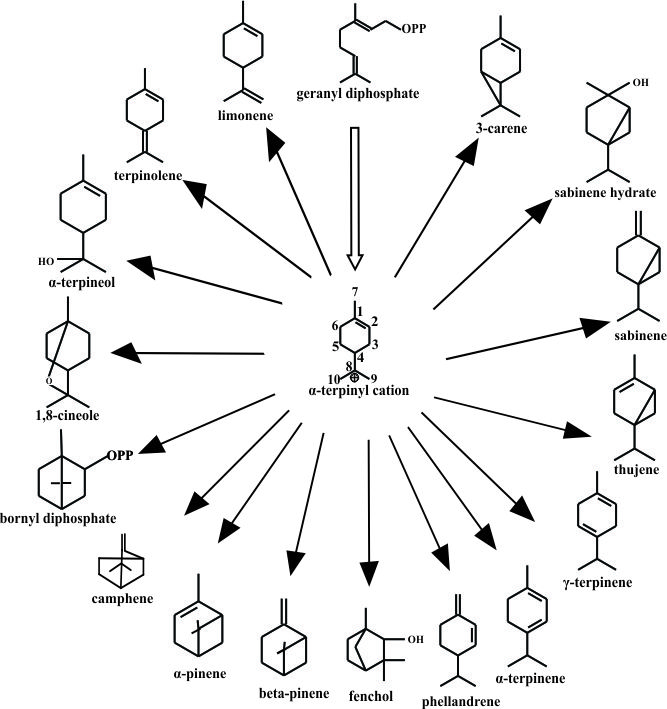
\includegraphics[width=.86\linewidth]{images/img.jpg}
	\caption{{ Exemplos do repertórios de monoterpenos produzidos pelas plantas por meio das ciclizações de Geranil Difosfato ($GPP$)}}
	\label{figIntroCarbocation}
\end{figure}

Há duas diferentes diferentes classes de  (TerpS): Classe I e Classe II definidas cataliticamente por aminoácidos essenciais. As (TerpS) I convertem formas do tipo linear, all-trans, isoprenóides, geranil (C10)\nobreakdash-farnesil (C15)\nobreakdash-, ou geranil (C20)-difosfato em numerosas variedades de monoterpenos, sesquiterpenos, e diterpenos. As (TerpS) I ligam o substrato delas pela coordenação de um local catalítico de íon metálico divalente (usualmente um $Mg^{2+}$), consistindo de uma cavidade central formada na maior parte das vezes por $\alpha$-hélices antiparalelas. 
Este local catalítico tem um rico aspartato $DDxxD/E$ motif e frequentemente outro $NSE/DTE$ motif em sua porção C-terminal.
As TerpS II atuam acionando a protonação de GGPP que resulta em sucessivos formatos do tipo carbocátion e ciclizados, a exemplo,o copalyl-difosfato ($CPP)$. Nas TerpS II, o $DxDD$ motif (diferente do $DDxxD/E$ motif das TerpS I) catalisa a reação usando um cofator $Mg^{2+}$ para auxiliar a ligação e posição do substrato. A diversidade dos terpenos também podem ser influenciadas pelas mudanças de nucleotídeos nos alelos dos genes das TerpS.
Realizar a predição da função enzimática é particularmente desafiador quando se lida com a terpeno-sintases (TerpS) devido à sua capacidade de produzir numerosas cadeias carbônicas por meio da catalisação de rearranjos complexos de carbocátions. Assim, pode ser impreciso usar para a anotação somente a homologia de sequência primária. A anotação das TerpS pode ser melhorada explorando o espaço viável de ciclização, para se encontrar as combinações que correspondam aos padrões: {\it in vitro} ou {\it in vivo} da literatura. Esta abordagem também pode ser útil para salientar a engenharia metabólica dos terpenóides nas plantas.
Este trabalho apresenta uma abordagem computacional para gerar um espaço virtual de rede química simulando carbocátions de GPP catalisados por monoterpeno sintase, sendo organizado da seguinte forma: Section~\ref{Método} apresenta o método, explicando como a rede química é produzida, sua estrutura de dados e cruzamentos. Seção~\ref{Resultados} discute os resultados, comparando-os com outras abordagens, além de destacar as suas contribuições para a biologia molecular.
Finalmente, Seção~\ref{Conclusão} apresenta a conclusão e um esboço dos próximos passos para que a abordagem seja consolidada como uma ferramenta para a comunidade científica.

%Este modelo foi produzido a partir do modelo de monografia do \href{https://github.com/UnB-CIC/Monografia}{Departamento de Ciência da Computação da UnB}.%

%Para citar assim:~\citep{Silva2018graph}, Escreva assim:%

\begin{verbatim}
~\citep{Silva2018graph}
\end{verbatim}

Para citar assim:~\cite{Silva2018graph}, Escreva assim:

\begin{verbatim}
~\cite{Silva2018graph}
\end{verbatim}


\section*{Objetivo}

Objetivos normalmente iniciam-se com verbos no infinitivo, por exemplo: 

Escrever um bom TCC.

\subsection*{Objetivos Específicos}

\begin{enumerate}
	\item Fazer AAAA
	\item Implementar BBBB
	\item Produzir CCCC
\end{enumerate}

Alguns cuidados devem ser tomados para melhorar a experiência do leitor.
O primeiro deles é sempre usar referências cruzadas de siglas, capítulos e seções, figuras e tabelas.
O nome a seguir: \acf{IFG}, é um exemplo de uso de siglas para ser usado na primeira citação.
\ac{IFG} é apenas a sigla, após seu primeiro uso.
Este é um exeplo de nota de rodapé\footnote{\url{https://www.capes.gov.br/images/stories/download/diversos/OrientacoesCapes_CombateAoPlagio.pdf}}.

\section{Descrição Dos Capítulos}

A última parte da introdução é uma descrição do que o leitor encontrará em cada capítulo.
Por exemplo, no \nameref{Referencial_Teorico} são apresentados comandos em \LaTeX e dicas para formatar seu TCC.
No \nameref{Metodo} é descrito o método utilizado para alcançar os objetivos listados aqui.
O \nameref{Resultados} apresenta os resultados obtidos.
No \nameref{Conclusao}, são apresentadas as conclusões, contribuições científicas e trabalhos futuros.



\chapter{Referencial Teórico}
\label{Referencial_Teorico}


Este capítulo oferece sugestões para descrever o referencial teórico.

\section{O que devo escrever aqui?}%

Descreva aqui tudo que for pertinente a seu trabalho com o máximo de detalhes e citando as respectivas fontes.

Você pode organizar este capítulo em seções:

\begin{verbatim} \section \end{verbatim}

e subseções: 

\begin{verbatim} \subsection \end{verbatim}
\chapter{Método}
\label{Metodo}
\indent
Degenhardt~\textit{et al.} descreveu mecanismos de reações para sintase de mono e sesquiterpenos das plantas, identificando diversos monoterpenos como produtos destas reações químicas. Baseado nesse periódico e outras fontes de ciclização enzimática de GPP, nós estendemos a abordagem apresentada por Silva~\textit{et al.}, de biossíntese de sesquiterpenos nas plantas, para monoterpenos.
O método formalmente modela reações químicas em um nível mecanístico, o qual forma caminhos que são dispostos como uma rede química. A rede química é abstraída como um hipergrafo orientado, em que os vértices correspondem a moléculas  e  hiperarestas a reações. Cada vértice representa uma molécula, que é abstraída para um grafo não orientado, no qual átomos são vértices e ligações são arestas. Em outras palavras, cada vértice da rede química é composto de um grafo não orientado, que representa uma molécula, e as reações químicas nessas moléculas são modeladas como transformações de grafos. 
Transformações de grafos baseadas em regras podem ser descritas formalmente pela gramática de grafos que generalizam muito mais sistemas de reescrita comumente utilizados. Cada regra descreve uma \emph{classe}  específica de reações químicas, como um fechamento de um átomo $C_1$ para $C_6$ ou um allyl shift. Cada regra possui um padrão $L$ de átomos e ligações que precisam estar presente nos educts para a reação correspondente acontecer. A parte correspondente é, assim, transformada conforme a regra foi especificada.Usamos o formalismo double pushout \emph{double pushout} (DPO) para reescrita de grafos porque ele é particularmente adequado para modelagem química: garante a reversibilidade da transformação e apoia bem o mapeamento de átomos. Aqui, cada regra tem o formato $p = (L \xleftarrow{l} K \xrightarrow{r} R)$  no qual $L$ é o grafo esquerdo, $R$ é o grafo direito e $K$ é o grafo de contexto. Morfismos de grafo $l$ e $r$ descreve a incorporação do contexto, dentro de L e R conectando esses grafos por $l\colon K\to L$ and $r\colon K\to R$.
Se uma regra $p$ é aplicada para um grafo $G$, é obrigatório  que $L$ “corresponda” a uma parte de $G$. A existência de outro morfismo de grafo ($m\colon L\to G$) retem essa informação, e junto com a regra $p$ e o morfismo $m$, define a transformação do substrato $G$ para o produto $H$, escrito como $G\xRightarrow{p,m}H$. A figura~\ref{figRuleExample} mostra um exemplo de uma regra de resfriamento pela água, em que as moléculas ($H_2O$ and $\alpha$-terpinol) a regra e o morfismo correspondente são expostos de acordo com a transformação de grafo DPO.

\begin{figure}[htbp]
	\centering
	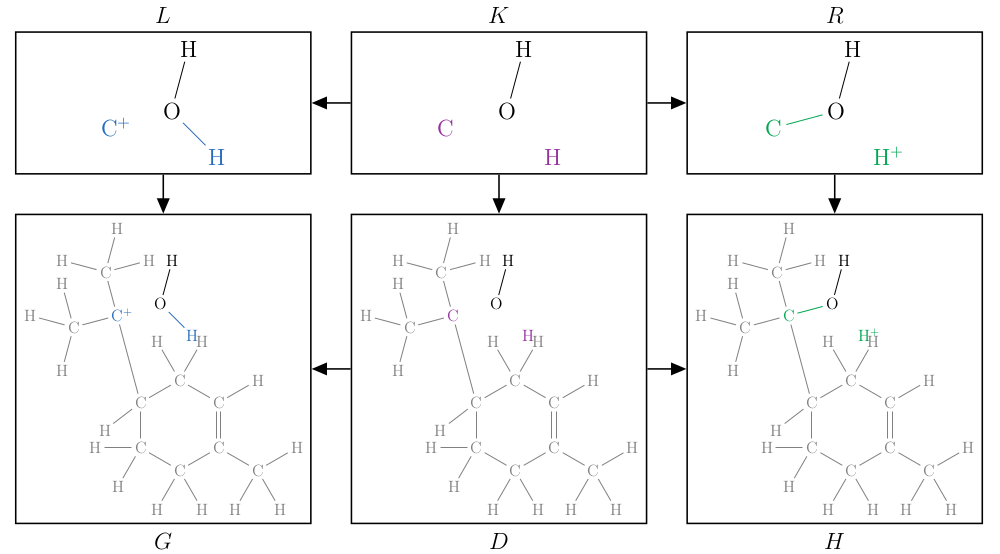
\includegraphics[width=\linewidth]{images/quenchingByWater.png}
	\caption{{Exemplo de regra por resfriamento de água e sua aplicação às moléculas $H_2O$ e $\alpha$-terpinol.}}
	\label{figRuleExample}
\end{figure}


\texttt{Med{\O}lDatschgerl}, ou  sua abreviação, \texttt{M{\O}D}, é um pacote de software inspirado quimicamente na transformação de grafo que pode direcionar um conjunto de moléculas iniciais e gerar a rede de reação química automaticamente, aplicando-se a regra baseada na transformação de grafos.  O conjunto de 17 regras de transformação de grafos, conforme as figuras abaixo, foi desenvolvido no formato GML para representar cada mecanismo de reação química encontrado na literatura. 
Essas regras transformam o conjunto inicial de moléculas ($GPP$ e $H_2O$) combinando-as em um primeira iteração, e gerando um novo conjunto de moléculas quimicamente possível. Então, em uma nova iteração, o conjunto de regras é novamente aplicada ao novo conjunto de compostos, gerando uma terceiro conjunto de compostos e assim por diante. Em cada simulação, é possível customizar ambos os conjuntos de regras a serem aplicados e o número de iterações. Para facilitar essa tarefa, construímos um interface Web, que trabalha offline e permite gerar um arquivo com o código de simulação de acordo com os parâmetros escolhidos. Um explicação gráfica para o método proposto é mostrado na figura ~\ref{figMethodSummary}.

\begin{figure}[H]
	\centering
	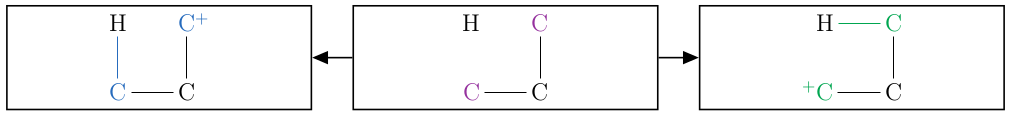
\includegraphics[width=.86\linewidth]{images/r1.png}
	\caption{\href{https://github.com/waldeyr/2PathTerpenes/blob/master/rules/1-3Hshift.gml}{1,3 hydrid shift.}}
	\label{figRule}
\end{figure}

\begin{figure}[H]
	\centering
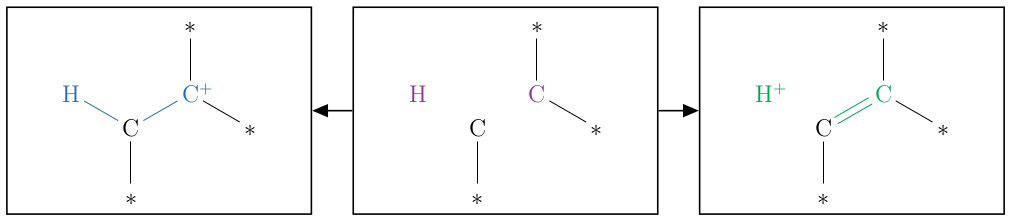
\includegraphics[width=.925\textwidth]{images/r2.png}
\caption{\href{https://github.com/waldeyr/2PathTerpenes/blob/master/rules/h_loss.gml}{Perda de $H^+$.}}
\label{figRule2}
\end{figure}

\begin{figure}[H]
	\centering
	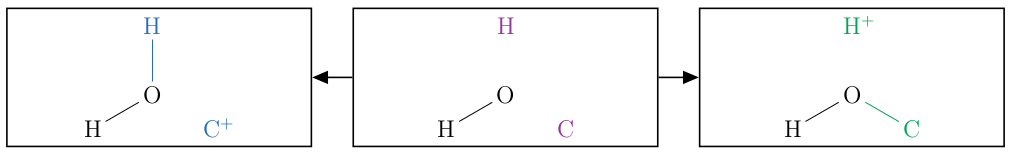
\includegraphics[width=.925\textwidth]{images/r3.png}
	\caption{\href{https://github.com/waldeyr/2PathTerpenes/blob/master/rules/h2o_gain.gml}{Captura de $H_2O$.}}
	\label{figRule3}
\end{figure}


\begin{figure}[H]
	\centering
	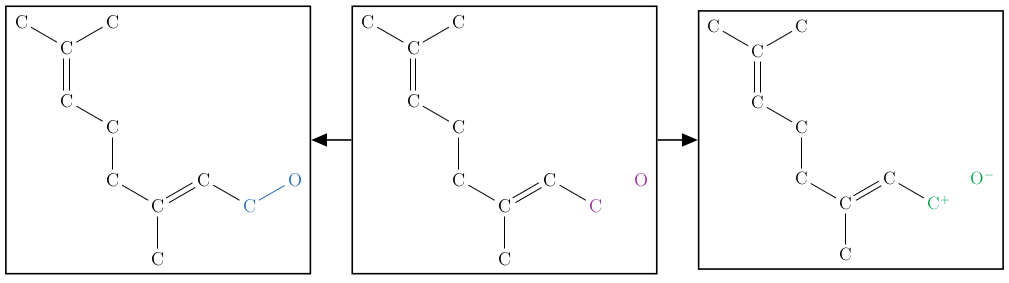
\includegraphics[width=.925\textwidth]{images/r4.png}
	\caption{\href{https://github.com/waldeyr/2PathTerpenes/blob/master/rules/opp_loss_gpp.gml}{Perda do GPP difosfato}}
	\label{figRule4}
\end{figure}

\begin{figure}[H]
	\centering
	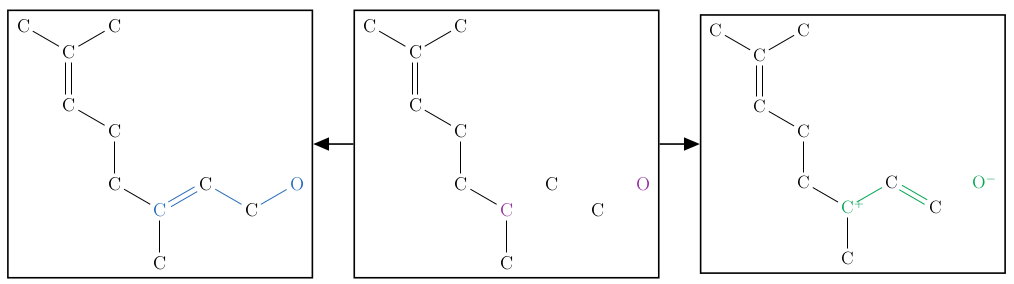
\includegraphics[width=.925\textwidth]{images/r5.png}
	\caption{\href{https://github.com/waldeyr/2PathTerpenes/blob/master/rules/opp_loss_gpp_alternative.gml}{Perda alternativa do difosfato GPP.}}
	\label{figRule5}
\end{figure}

\begin{figure}[H]
	\centering
	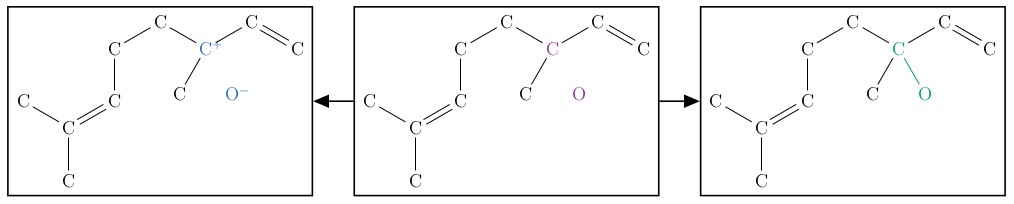
\includegraphics[width=.925\textwidth]{images/r6.png}
	\caption{\href{https://github.com/waldeyr/2PathTerpenes/blob/master/rules/opp_gain_by_geranyl_cation.gml}{Caotura de difosfato pelo geranil cátion}}
	\label{figRule6}
\end{figure}

\begin{figure}[H]
	\centering
	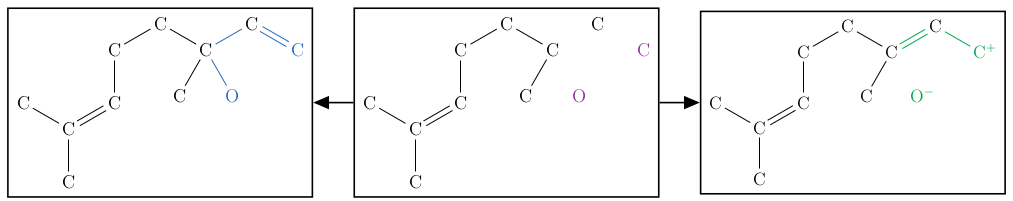
\includegraphics[width=.925\textwidth]{images/r7.png}
	\caption{\href{https://github.com/waldeyr/2PathTerpenes/blob/master/rules/opp_loss_for_lpp_c3.gml}{Perda do difosfato LPP.}}
	\label{figRule7}
\end{figure}

\begin{figure}[H]
	\centering
	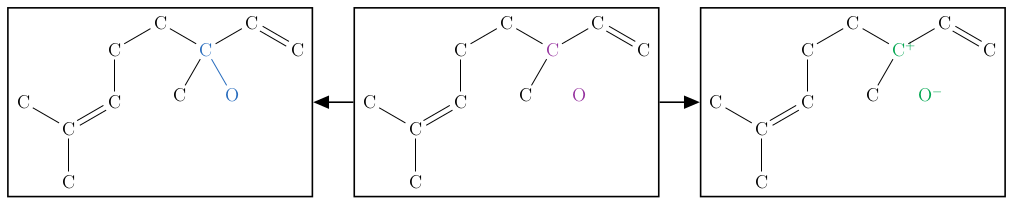
\includegraphics[width=.925\textwidth]{images/r8.png}
	\caption{\href{https://github.com/waldeyr/2PathTerpenes/blob/master/rules/opp_loss_for_lpp_c3_alternative.gml}{Perda alternativa do difosfato LPP.}}
	\label{figRule8}
\end{figure}


\begin{figure}[H]
	\centering
	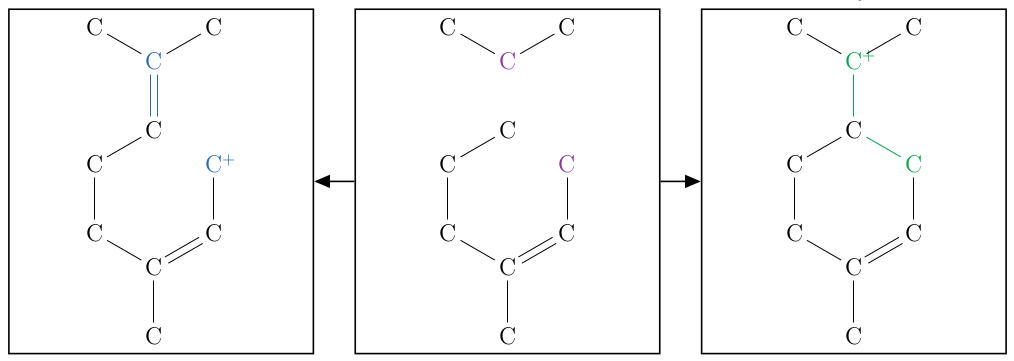
\includegraphics[width=.925\textwidth]{images/r9.png}
	\caption{\href{https://github.com/waldeyr/2PathTerpenes/blob/master/rules/1-6-closure.gml}{Fechamento do anel 1-6.}}
	\label{figRule9}
\end{figure}


\begin{figure}[H]
	\centering
	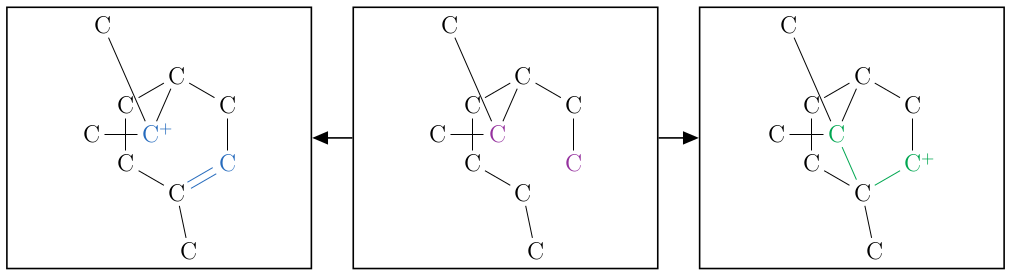
\includegraphics[width=.925\textwidth]{images/r10.png}
	\caption{\href{https://github.com/waldeyr/2PathTerpenes/blob/master/rules/3\%2C7-closure.gml}{Fechamento do anel 3-7.}}
	\label{figRule10}
\end{figure}


\begin{figure}[H]
	\centering
	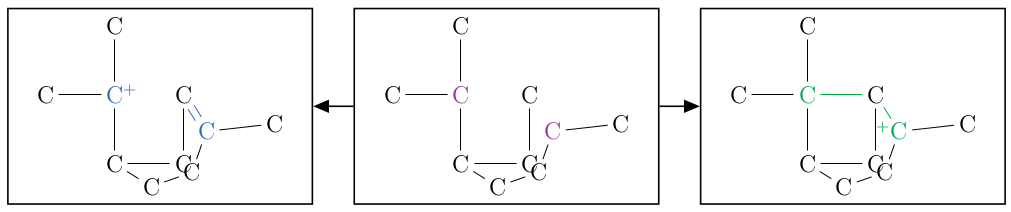
\includegraphics[width=.925\textwidth]{images/r11.png}
	\caption{\href{https://github.com/waldeyr/2PathTerpenes/blob/master/rules/2\%2C7-closure.gml}{Fechamento do anel 2-7.}}
	\label{figRule11}
\end{figure}


\begin{figure}[H]
	\centering
	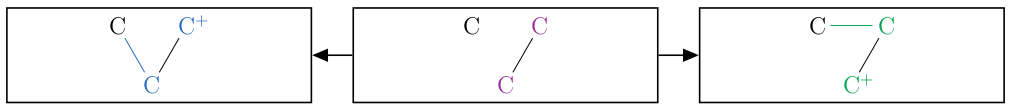
\includegraphics[width=.925\textwidth]{images/r12.png}
	\caption{\href{https://github.com/waldeyr/2PathTerpenes/blob/master/rules/WMshift.gml}{Wagner-Meerwein 1,2 alcyl shift}}
	\label{figRule12}
\end{figure}

\begin{figure}[H]
	\centering
	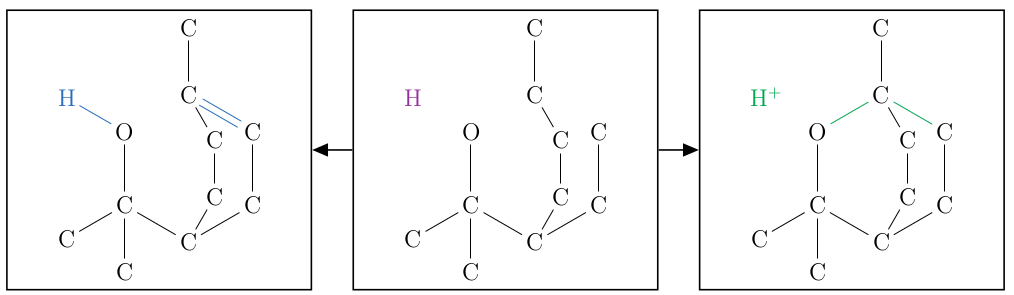
\includegraphics[width=.925\textwidth]{images/r13.png}
	\caption{\href{https://github.com/waldeyr/2PathTerpenes/blob/master/rules/1-8-cyc.gml}{Ciclização 1-8}}
	\label{figRule13}
\end{figure}


\begin{figure}[H]
	\centering
	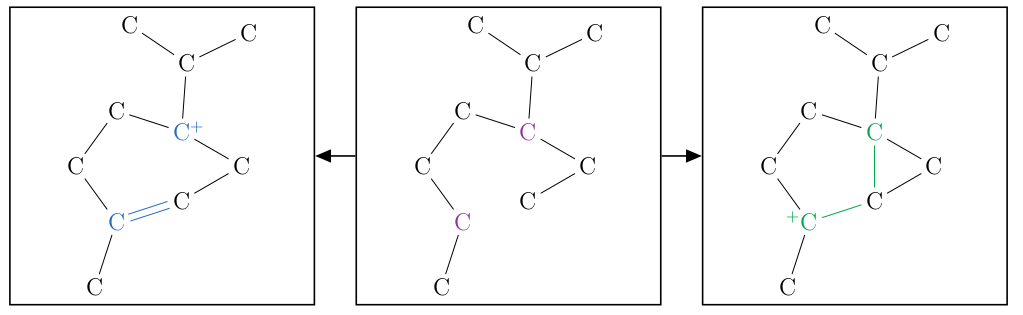
\includegraphics[width=.925\textwidth]{images/r14.png}
	\caption{\href{https://github.com/waldeyr/2PathTerpenes/blob/master/rules/2-6-closure.gml}{Fechamento 2-6}}
	\label{figRule14}
\end{figure}

\begin{figure}[H]
	\centering
	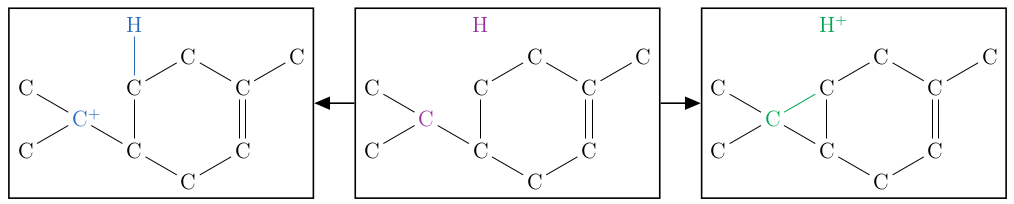
\includegraphics[width=.925\textwidth]{images/r15.png}
	\caption{\href{https://github.com/waldeyr/2PathTerpenes/blob/master/rules/5-7-closure.gml}{Fechamento 5-7}}
	\label{figRule15}
\end{figure}

\begin{figure}[H]
	\centering
	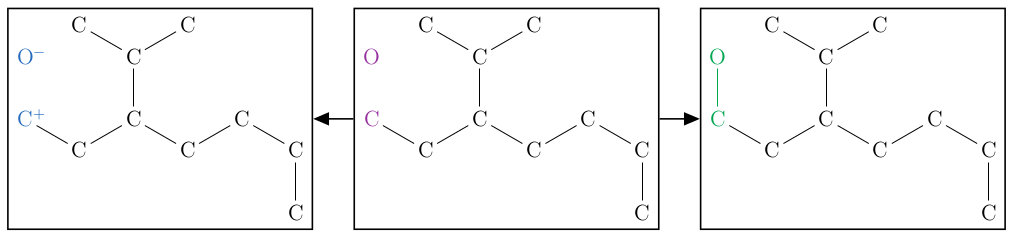
\includegraphics[width=.925\textwidth]{images/r16.png}
	\caption{\href{https://github.com/waldeyr/2PathTerpenes/blob/master/rules/opp_gain_by_bornyl_cation.gml}{Captura de difosfato pelo bornil cátion.}}
	\label{figRule16}
\end{figure}

\begin{figure}[H]
	\centering
	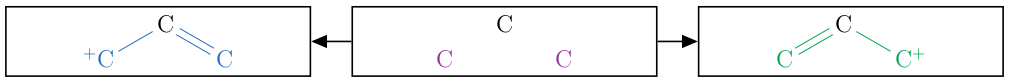
\includegraphics[width=.925\textwidth]{images/r17.png}
	\caption{\href{https://github.com/waldeyr/2PathTerpenes/blob/master/rules/allylshift.gml}{Allylic charge shift}}
	\label{figRule17}
\end{figure}


\begin{figure}[htbp]
	\centering
	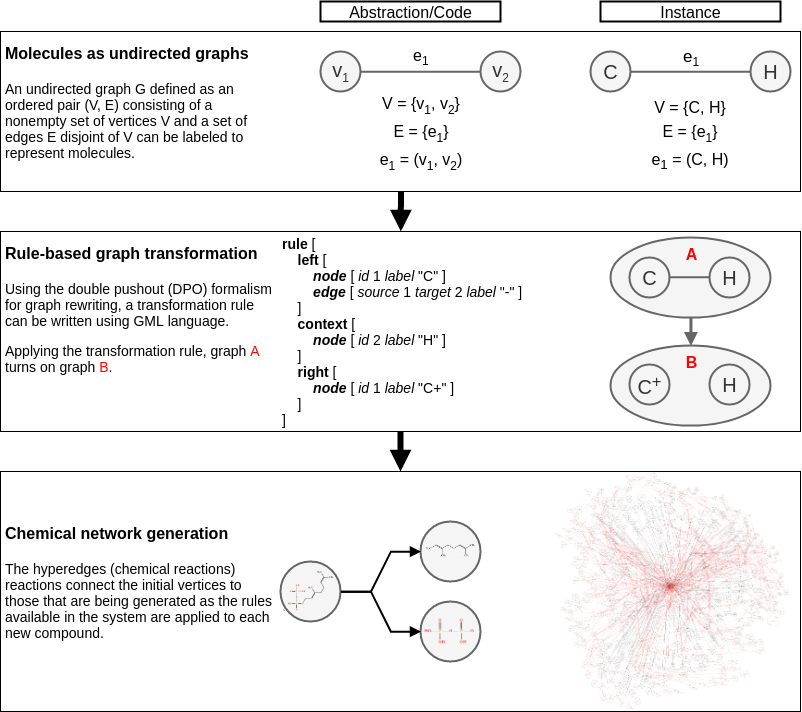
\includegraphics[width=\linewidth]{images/BIBM2019DanielaMethod.png}
	\caption{{Método resumido com exemplos de códigos/abstrações e suas aplicações para geração da rede química baseada nas transformações de grafos.}}
	\label{figMethodSummary}
\end{figure}


%\section{O que devo escrever aqui?}%

%Cada ferramenta, tecnologia, definições e todo o arcabouço teórico do trabalho deve estar em seu \nameref{Referencial_Teorico}.%
%Aqui, no \nameref{Metodo} você deve escrever como utilizou as ferramentas, tecnologias e outros recursos para resolver o problema proposto com vistas a alcançar seus objetivos.%
%Este não é lugar para definir nada novo.%


%Não caia na tentação de dizer aqui os resultados! Guarde-os para o \nameref{Resultados}. Muitas vezes é interessante começar a escrita, justamente pelo \nameref{Resultados}.%

%\fontshape{n}\selectfont%
%A tabela com a listagem de todas as atividades, pontuação e somatório encontra se na página de finalização do formulário.%


\chapter{Resultados e discussões}
\label{Resultados}

Baseada na ciclização enzimática de GPP, nossas simulações foram aptas a gerar todos os componentes dispostos na figura ~\ref{figIntroCarbocation}. Junto com esses componentes, as simulações produzem um vasto montante de outros componentes acompanhados por todas as ciclizações e intermediários dos quais eles originam, formando uma extensa rede química de potenciais produtos de terpenos. Toda rede química pode ser convencionalmente exportada para um documento PDF.  Também, o hipergrafo, que é em si a própria rede química, pode ser computacionalmente acessado e processado para futuras análises. Além disso, é possível armazenar a rede química usando um banco de dados em grafos, como descrito em ~\cite{Silva2018graph}. Apesar de as simulações serem customizadas, o código fonte escrito pode não ser trivial para pesquisas não computacionais. A interface Web criada atenua esta condição, fazendo a customização da simulação mais intuitiva e menos capciosa, sendo suficientes alguns “drag and drop” e cliques.   Essa interface, combinada com uma imagem do Docker com todo o ambiente preparado, está disponível no \href{https://github.com/waldeyr/2PathTerpenes}{GitHub}\footnote{https://github.com/waldeyr/2PathTerpenes}.

\section{Percepções sobre a rede química gerada}

A combinação das regras de transformação de grafos e o número de iterações permitem explorar um amplo espaço químico possível de monoterpenos, expondo todos os mecanismos de ciclização enzimática de seu precursor, o GPP. Notavelmente, neste espaço químico, há três grupos de monoterpenos: os que são encontrados na natureza e são conhecidos, os que são encontrados na natureza, mas permanecem desconhecidos; e os que são fisicamente possíveis, mas provavelmente não serão encontrados na natureza devido ao alto custo de energia para sua produção. 

Avanços científicos na tecnologia como espectometria de massas combinada com cromatografia gasosa tem possibilitado a alocação de mais e mais monoterpenos do primeiro grupo, isto é, dos que são conhecidos. Outras tecnologias como engenharia genética tem possibilitado experimentos de diversas hipóteses na diversidade e rendimento da produção de monoterpenos nas plantas. É possível alterar a viabilidade do perfil de monoterpenos das plantas, como demonstrado por  Krasnyanski et al. no trabalho pioneiro deles com hortelã-pimenta, seguido por muitos outros como Lucker et
al., alcançando a produção de monoterpenos introduzindo TerPS de limão em plantas de tabaco. Fatores como a avaliabilidade do GPP, compartimentação subcelular, crescimento de plantas e custos físicos são problemas relevantes a serem considerados para engenharia metabólica das plantas. Como muitos fatores além da sequência primária influenciando o perfil de monoterpenos de uma TerpS, manter metadados sobre vias químicas é relevante para possibilitar a identificação de cenários da biossíntese de monoterpenos sob certas condições. Descobrir as possibilidades da produção de monoterpenos de acordo com determinadas circunstâncias pode ser útil para preditar a função das TerpS e consequentemente para engenharia metabólica das plantas.  Isso poderia ajudar a responder importantes questões biológicas, a exemplo: seria possível prever quais alterações seriam feitas ao modificar o perfil de monoterpenos de uma enzima comparando-a a um grupo de TerpS que produz a mesma variedade de monoterpenos? 


Terpenóides têm muitas aplicações, tanto ecológicas quanto comerciais, que são evidenciadas pelas características como moléculas voláteis influenciando o comportamento de insetos. 
A engenharia de produção de terpenóides nas plantas tem o potencial de melhor produzir o manejo de pragas ou polinização aprimorada, por exemplo. 

\section{Comparação com trabalhos relacionados}

Há algumas iniciativas de predições relevantes de vias metabólicas computacionais que consideram transformações intermediárias em reações químicas como  as RetroRules, Biotransformer, Isegawa et al., and Tian et al. Apesar de fornecerem resultados comparáveis, essas abordagens diferem uma das outras por usar distintos métodos e estrutura de dados para representar as moléculas. RetroRules e Biotransformer usam descrições de reações químicas codificadas por SMARTS e SMIRKS. Isegawa et. al. usaram o método AFIR para prever computacionalmente o caminho para formação de terpenos. Tian et al. apresentaram uma abordagem computacional para gerar todos os possíveis carbocátions da sínteses de monoterpenos definindo e organizando o espaço químico produzido. Esse trabalho tem objetivos e resultados similares a RetroRules, Biotransformer, and Tian et al., mas sua metodologia é bastante diferenciada. Chow et al. usou a abordagem de Tian et al. [6] para caracterizar a sintase de sesquiterpeno de Streptomyces clavuligerus, que colabora com a ideia que as redes químicas podem ajudar as tarefas funcionais das TerpS.


%\section{O que devo escrever aqui?}%
%Bem, quando você iniciou seu trabalho, você tinha um problema claro a resolver.%
%Você pesquisou a respeito do seu problema e também a respeito de ferramentas, tecnologias e outros recursos que poderiam ajudá-lo a resolver seu problema. No método você estabelecu os passos usados para resolver o problema. Agora é hora de mostrar em detalhes que você alcançou os objetivos definidos na \nameref{Introducao}.%

%Oriente-se pelos Objetivos. Descreva em detalhes o seu sucesso!!%
\chapter{Conclusão}
\label{Conclusao}

O método proposto neste trabalho provê uma forma valiosa para explorar a diversidade de monoterpenos expondo todo o processo de sua produção em uma estrutura de dados computacionalmente tratável. Ademais, a opção de salvar a rede química em um banco de dados torna-se assim particularmente interessante se estes metadados são armazenados juntos, o que faz ser possível explorá-los através de consultas. O uso de banco de dados em grafos para fins biológicos, embora recente, já está bem estabilizado com casos de grande sucesso. Além dos resultados aqui reportados, este trabalho traz um esboço de um sistema capaz de modelar uma rede química computacional e evidência da literatura experimental como metadados para melhor guiar a tarefa funcional das Terps. Tal sistema é um trabalho futuro que substituirá o banco de dados 2Path.


% References

\begin{references}
  \bibliography{bib/references}
\end{references}

% Appendix
\theappendix



\end{document}
